%%%%%%%%%%%%%%%%%%%%%%%%%%%%%%%%%%%%%%%%%%%%%%%%%%%%%%%%%%%%%%%%%%% 
%                                                                 %
%                            CHAPTER Three                        %
%                                                                 %
%%%%%%%%%%%%%%%%%%%%%%%%%%%%%%%%%%%%%%%%%%%%%%%%%%%%%%%%%%%%%%%%%%% 
 
\chapter{SEMANTIC IMPORTANCE} 
\blfootnote{Portions of this chapter previously appeared as: Rui Yan, Mark T Greaves, William P. Smith, Deborah L. McGuinness 2016. ``Remembering the Important Things: Semantic Importance in Stream Reasoning." Stream Reasoning 2016 Workshop, International Semantic Web Conference 2016} 
Timely producing query results from processing infinite streams requires efficient methods.
Usually, the answers to a query are hidden in the heterogeneous streams where not all of the data items are used \cite{mileo2013streamrule}. 
An ideal scenario is where all the data items contain the necessary information for answering the query.
For example, registering the query ``select ?s ?p ?o where \{?s ?p ?o\}'' in the stream yields all the streaming data.
Speaking from a practical perspective, this ideal scenario is not common, thus it becomes very critical to employ some efficient algorithms to produce timely and correct outputs from stream reasoning applications.

Streaming data is processed with a window, whose view of the entire data stream is limited by the window size. 
Even though some systems maintain a synopses of the overall stream, the synopses will grow in size as time goes by, which can increasingly consume the storage and computing resources. 
Thus, there is a need for smart and flexible window management strategies that allow identifying, preserving the necessary data items as well as evicting unnecessary data items in the window. 
The strategies also need to be computationally cheap and easy to implement. 

This chapter introduces the notion of semantic importance, which models the importance of the streaming data from its various orderings.
It also covers how window management strategies can be created with semantic importance, as well as how system performance is positively affected by semantic importance. 
%
\section{Semantic Importance}

\begin{figure}[!htbp]
	\centering
	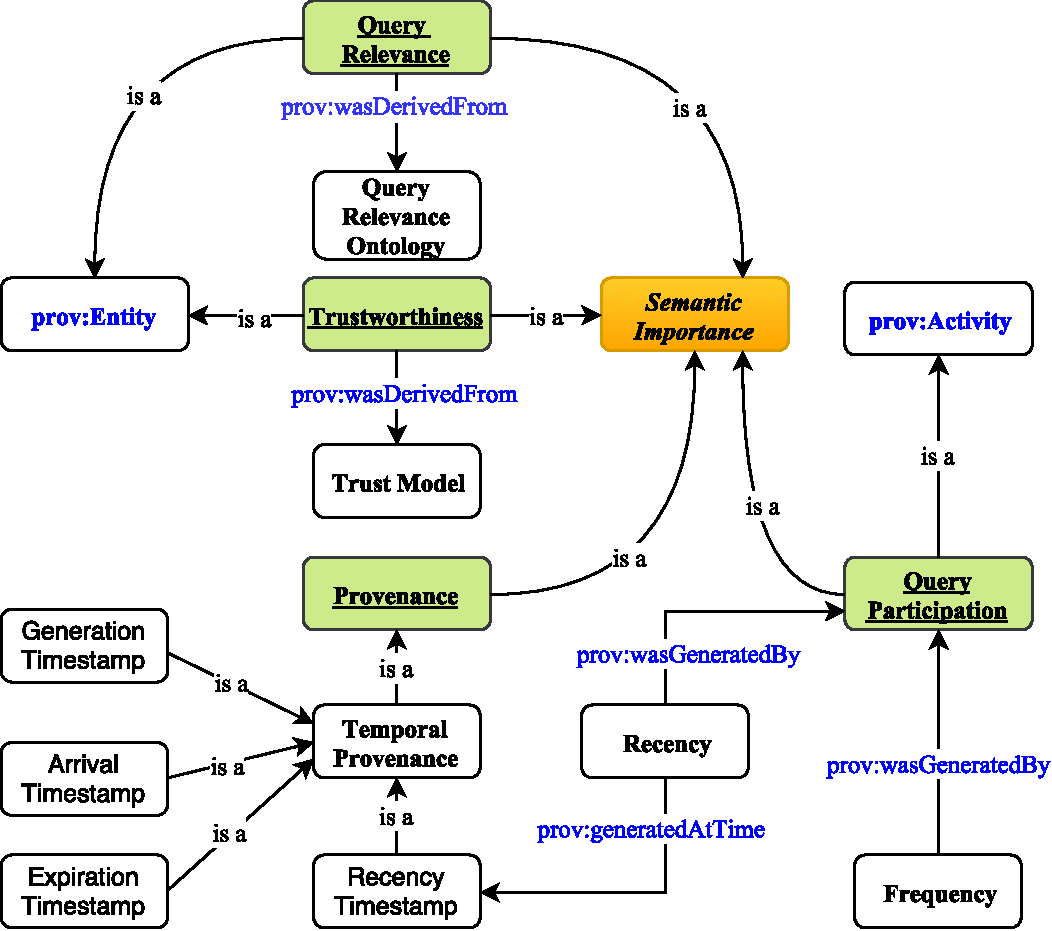
\includegraphics[width=5in]{img/3-si.pdf}
	\caption{Semantic Importance Conceptual Model}
	\label{fig:3-si} 
\end{figure}

For the concept of semantic importance to be relevant, it needs to be the case that not all of the data in the window will contribute equally to the query result \cite{mileo2013streamrule}. 
Given this, the ability to specifically identify the most important data and utilize it effectively is critical for improving stream reasoning system performance. 
So, the question is, can we differentiate and identify effective metrics for use in enabling this task? 
Specifically, in Figure \ref{fig:1-seew}, in order to get the correct answer at $t_{2}$, we need to find a principled and general way to keep $\largetriangleup_{A}$, $\times^{\circ}_{A}$ and wait for $\largecircle_{A}$ to arrive. 
Determining that $\largetriangleup_{A}$, $\times^{\circ}_{A}$ and $\largecircle_{A}$ are more important than other data items is an intuitive observation for a human to make. 
Our goal is to formalize certain parts of this task of judging the relative importance of different streaming data items and use those as the foundation of an ordering relation that can be used for window management.
To do this, I present semantic importance.

\textbf{Semantic importance is defined as an extensible conceptual model that describes the importance of the streaming data by leveraging various streaming data orderings.}
re
Such data orderings are not limited to logical orderings, but also query participation, provenance, and trustworthiness, etc. 
Semantic importance is represented in a priority vector \cite{saaty2003decision}, with elements ordered according to a preference function.
For example, priority vector $V_{p} = [x, y, z]$ has three elements $x, y,$ and $z$.
$x$ is preferred to $y$, and $x, y$ is each preferred to $z$.
The lefter the element is placed, the more preferential the element is.  
There is no restriction on the number of vector elements. 
The traits of the priority vector allow us to consider multiple semantic importance metrics simultaneously while preserving the ability to prioritize some selecting metrics. 

Figure \ref{fig:3-si} shows the conceptual model of semantic importance. 
This conceptual model leverages some concepts from Prov-O \cite{lebo2013prov} to describe the inter-class relationships. 
It is modeled by data orderings, which currently include four aspects: provenance, query participation, trustworthiness, and query relevance.
Each aspect will be introduced in details below.
%
\subsection{Provenance}

\begin{figure}[!htbp]
	\centering
    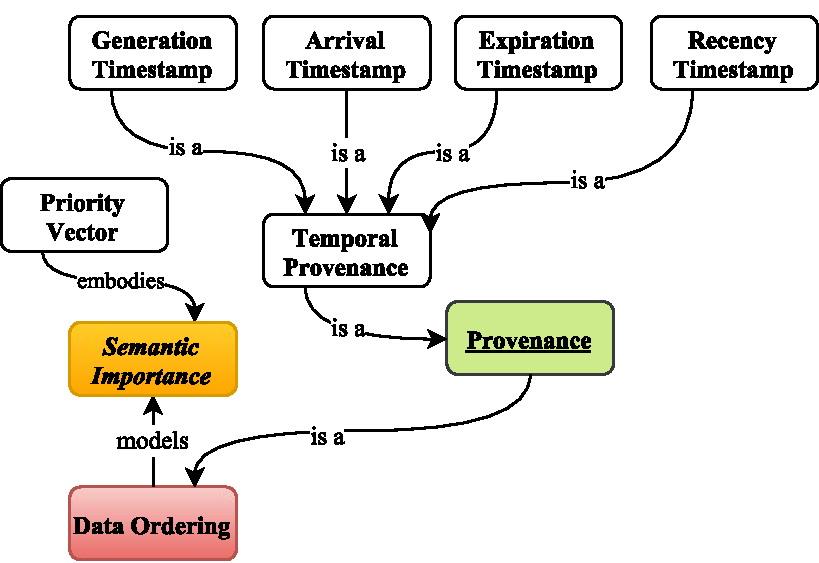
\includegraphics[width=5in]{img/3-sip.pdf}
    \caption{Semantic Importance - Provenance}
    \label{fig:3-sip}
\end{figure}

Provenance is a factor in judging the importance of a streaming data item \cite{gao2010survey}.
This dissertation takes its definition from a foundation paper \cite{ram2009new} in data provenance, 
where \textbf{``provenance is defined as a set of n-tuples: what, when, where, how, who, which, and why.''}
There are several alternate definitions, but this one will suit the dissertation goal since it is a representative definition that includes the extensibility with other definitions. 
It provides the directions to extend provenance aspect with other perspectives such as ``what'', ``where'' or ``how''. 
In the current model, logical provenance\footnote{It is also referred as temporal provenance.} is included and is corresponding to ``when'' aspect in the definition.
This model can certainly go beyond that in the dissertation future work but ``when'' is really what should be started from, because I want to show it for the silent logical assumption.

Even though this dissertation focuses on ``when'' aspect, other types of provenance can also be expanded. 
For example, ``where'' can possibly include the geographical information of the data, whereas ``who'' can possibly refer to the agent that performs some actions. 
In Chapter 5, the soccer offside offense use case leverages positional data as the where-provenance, as well as the players' sensor id as who-provenance. 
The expansion of the provenance aspect will be as one of the future of this dissertation.

There are four branches following the logical provenance.
Generation timestamp ($\tau_{g}$) is assigned by the streaming source, and describes when the data is generated.
Arrival timestamp ($\tau_{a}$) is assigned by the processing system, and describes when the data arrives at the system.
Expiration timestamp ($\tau_{e}$) is assigned by either the processing system or the streaming source, and describes when the data expires.
Recency timestamp ($\tau_{qp}$) is assigned by the system, and is associated with the query participation recency.
For example, priority vector $[\tau_{a}]$ contains $\tau_{a}$ as the only aspect to describe the data importance, and this is the silent logical assumption.
$[\tau_{e}, \tau_{qp}, \tau_{a}]$ uses three aspects to describe the data importance. 
%
\subsection{Query Participation}

\begin{figure}[!htbp]
	\centering
    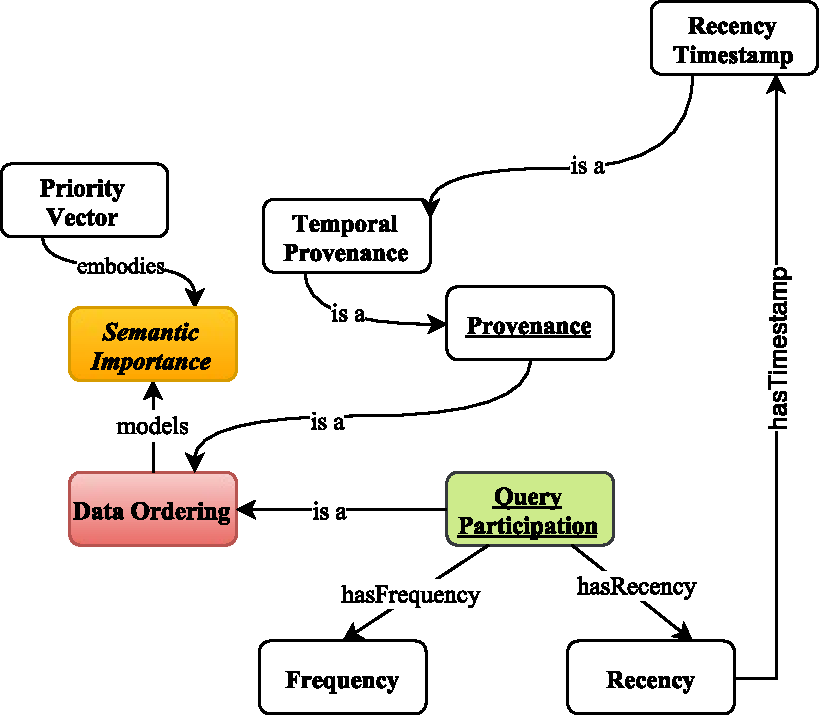
\includegraphics[width=5in]{img/3-siqp.pdf}
    \caption{Semantic Importance - Query Participation}
    \label{fig:3-siqp}
\end{figure}

\textbf{Query participation is defined as: data items participate in a query if they contain necessary information used by the query engine to return non-empty answers.}
Two query participation aspects are frequency and recency.
Frequency ($f_{qp}$) is an integer value that describes how many times a data item participates in the query, 
and recency ($\tau_{qp}$) is a timestamp that describes the most recent time-point for a data item participating in the query.

\begin{figure}[!htbp]
	\centering
    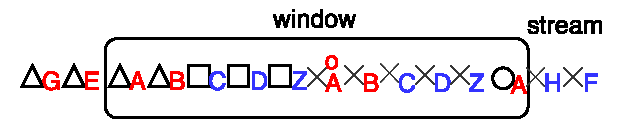
\includegraphics[width=5in]{img/3-siqpe.pdf}
    \caption{Query Participation Example}
    \label{fig:3-siqpe}
\end{figure}

To further explain the definition of query participation, let us consider the example in Figure \ref{fig:3-siqpe}.
We will continue to use the data stream of the soccer offside running example and Table \ref{tab:icons}. 
As mentioned in the previous section, Player A commits an offside offence if he/she is an attacker ($\largetriangleup_{A}$), is at offside position ($\times^{\circ}_{A}$) and involves in an active play ($\largecircle_{A}$) at some time point t.
At this point, since all of the necessary data items are present in the window, the query ``who commits an offside offence'' will be answered. 
This example illustrates that not all of the data items in the window will convey the necessary information that can be used to answer the query. 
The reason why the answer for the query is non-empty is because of the complete presence of $\largetriangleup_{A}$, $\times^{\circ}_{A}$ and $\largecircle_{A}$ at the current active window.
Thus, we say that $\largetriangleup_{A}$, $\times^{\circ}_{A}$ and $\largecircle_{A}$ participate in the query, while others (such as $\largetriangleup_{B}$, $\largesquare_{D}$ or $\times_{B}$) do not. 

\begin{table}[!htbp]
	\centering
    \caption{Updated Query Participation Frequency and Recency}
    \label{tab:uqpfr}
    \begin{tabular}{|c||c|c|c|c|c|c|c|c|c|c|c|} \hline
    	data item & $\largetriangleup_{A}$ & $\largetriangleup_{B}$ & $\largesquare_{C}$ & $\largesquare_{D}$ & $\largesquare_{Z}$ & $\times^{\circ}_{A}$ & $\times_{B}$ & $\times_{C}$ & $\times_{D}$ & $\times_{Z}$ & $\largecircle_{A}$ \\ \hhline{|=#=|=|=|=|=|=|=|=|=|=|=|}
		$f_{qp}$ & 1 & 0 & 0 & 0 & 0 & 1 & 0 & 0 & 0 & 0 & 1 \\ \hline
        $\tau_{qp}$ & $\tau_{qp1}$ & - & - & - & - & $\tau_{qp1}$ & - & - & - & - & $\tau_{qp1}$ \\ \hline 
    \end{tabular}
\end{table}

Assume that it is the first time to execute the query, thus all data items should have $f_{qp} = 0$, and no $\tau_{qp}$. 
When the query result is returned, data items' statistics will be updated. 
Table \ref{tab:uqpfr} shows that $\largetriangleup_{A}$, $\times^{\circ}_{A}$ and $\largecircle_{A}$'s $f_{qp}$ increases by 1, and $\tau_{qp}$ becomes $\tau_{qp1}$.
They have the same $\tau_{qp}$ because they participate in the query at the time $t = \tau_{qp1}$. 
Other data items' $f_{qp}$ and $\tau_{qp}$ remain unchanged. 
%
\subsection{Trustworthiness}

\begin{figure}[!htbp]
	\centering
    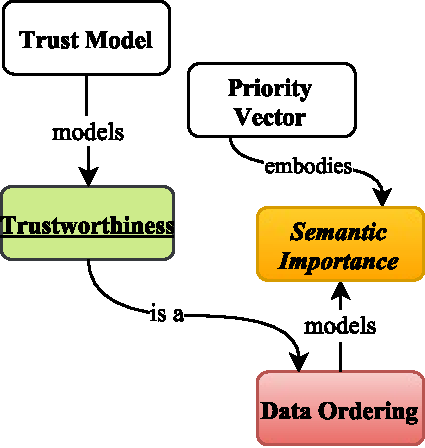
\includegraphics[width=5in]{img/3-sit.pdf}
    \caption{Semantic Importance - Trustworthiness}
    \label{fig:3-sit}
\end{figure}

Different work models trustworthiness in different ways.
For example, in \cite{bertino2009challenge}, trustworthiness is modeled as ``the probability of one data item to be correct''. 
Other work models data trustworthiness from perspectives of data quality \cite{juran1999quality}, \cite{kahn2002information}, \cite{prince2004semiotic}, \cite{wand1996anchoring}, semantic integrity \cite{date2004database} and reputation techniques \cite{kamvar2003eigentrust}, \cite{levien2009attack}. 
The concept of trustworthiness can be very broad, which makes it very suitable to be included in the semantic importance conceptual model. 
In this dissertation, \textbf{trustworthiness is defined as ``worthy of confidence''} \cite{trustdef2018}.
However, in order to let the concept of trustworthiness to be useful and comparable, this work relies on the related literatures on trustworthiness modeling. 

Semantic importance doesn't emphasize on any specific trust models.
But for the sake of convenient processing, data items should be stamped with a numerical value as a trust score ($t^{tm}_{s}$) by a selected trust model ($tm$). 
%
\subsection{Query Relevance}

\begin{figure}[!htbp]
	\centering
    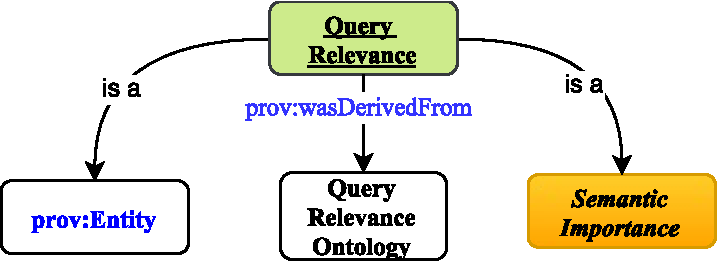
\includegraphics[width=5in]{img/3-siqr.pdf}
    \caption{Semantic Importance - Query Relevance}
    \label{fig:3-siqr}
\end{figure}
Query relevance ties specific knowledge about queries and data into window management using formal semantics. 
It is \textbf{defined as the description of data items' potential to answer the query}.
Query relevance shares the similar assumption from \cite{mileo2013streamrule}: 
``not all raw data from the input stream might be relevant for complex reasoning''.
This description is query-informed, and encoded in an ontology called ``query relevance ontology''.
The query relevance ontology is provided by the users, and enables query relevance as shown in Figure \ref{fig:3-siqr}.
For the concepts in the query relevance ontology to be useful, it is usually constructed with existing concepts in the background domain ontology, which is shown in Figure \ref{fig:3-siqreo}.

\begin{figure}[!htbp]
	\centering
    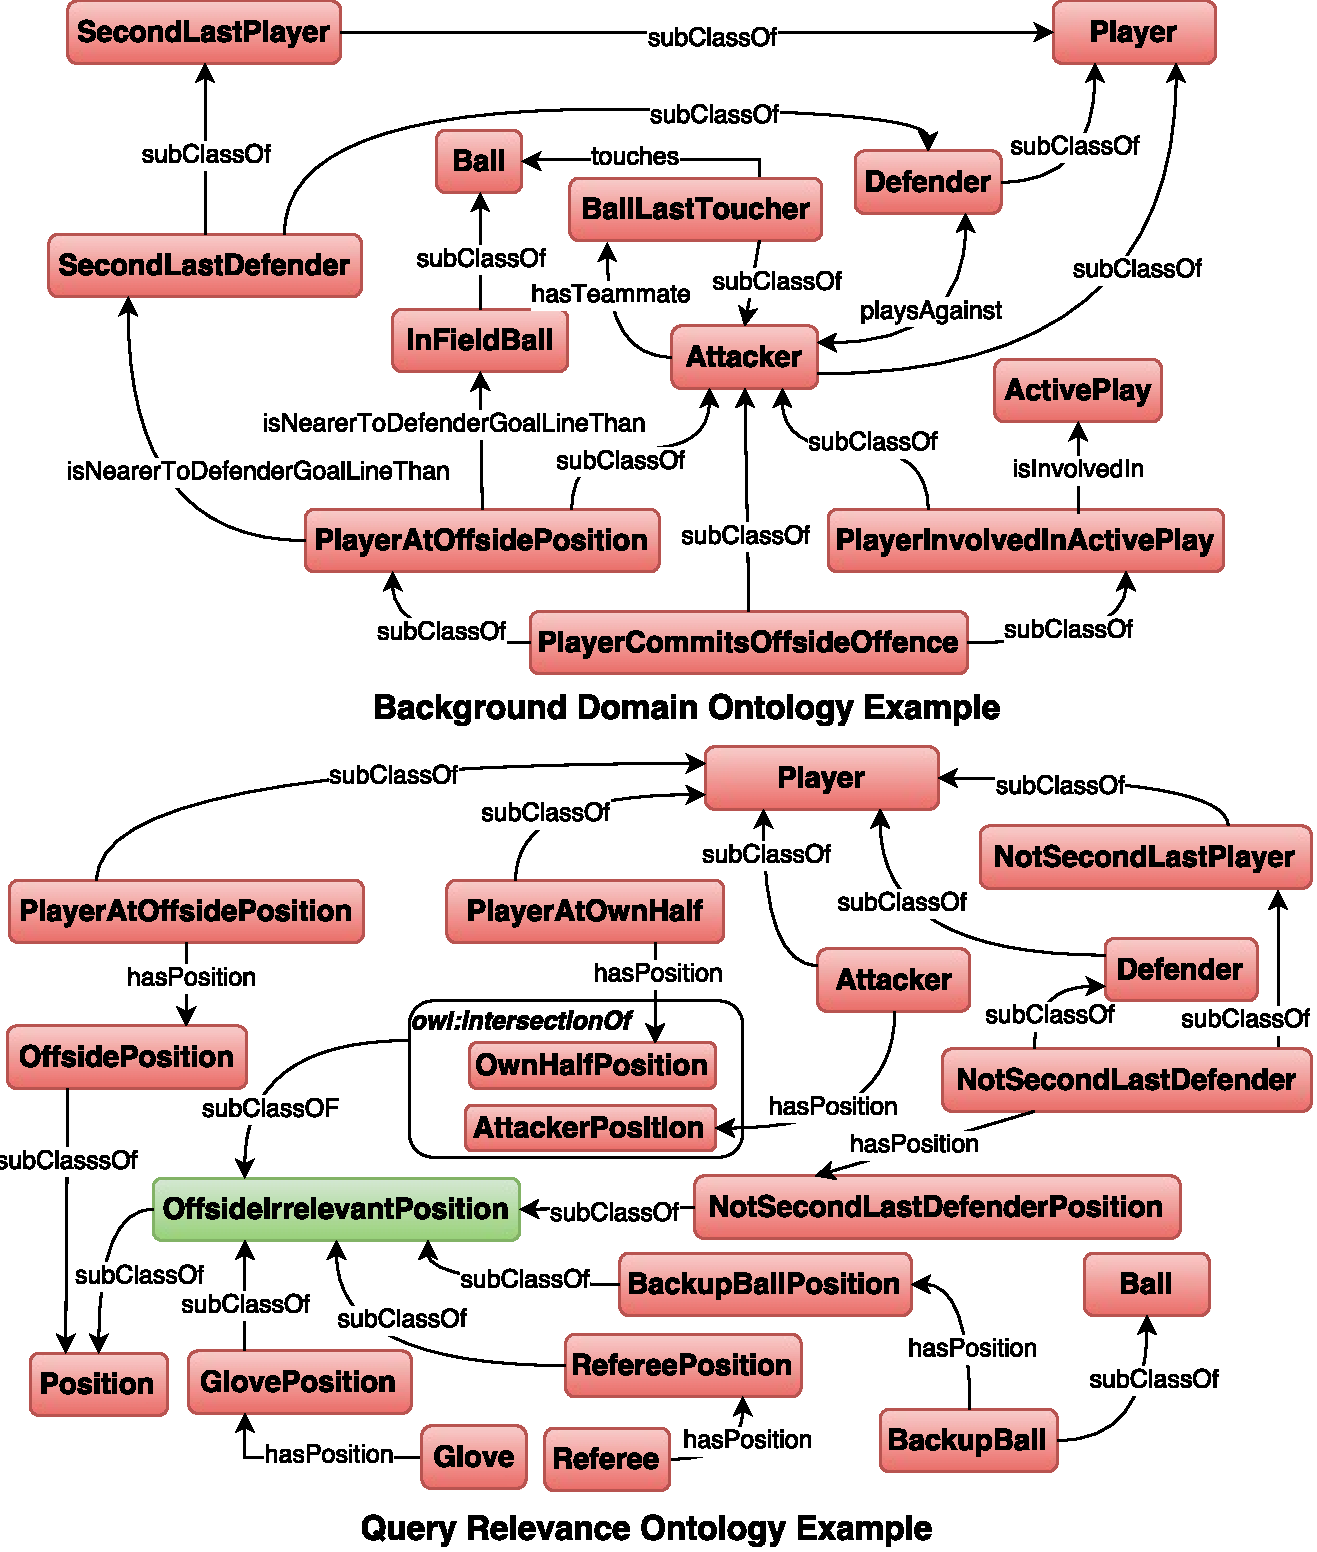
\includegraphics[width=5in]{img/3-siqreo.pdf}
    \caption{Query Relevance Ontology}
    \label{fig:3-siqreo}
\end{figure}

In Figure \ref{fig:3-siqreo}, all the red boxes are concepts encoded in the background domain ontology of soccer, which contains the general knowledge about the overall soccer domain. 
The background ontology can not only answer the query of ``who commits an offside offence'', but also ``who are attackers'', ``which team is controlling the ball'' and ``who is challenged by whom'', etc. 
the only concept in the query relevance ontology is marked in green, which is \textbf{OffsideIrrelevantPosition}. 
But the query relevance ontology only provides details of query relevance for one specific query, which in this case is ``who commits an offside offence''. 

In the Query Participation Section, we have already mentioned that not all of the data will be participating in the query.
The idea of query relevance is to encode the knowledge of human literacy about the query. 
In soccer offside detection, humans know that the positions of the offensive players at their own half will not participate in the query according to the soccer offside definition. 
It is easy to ignore such irrelevant data for linesmen during officiating the game since they are aware of this knowledge. 
However, in order to let the machines acquire this knowledge, users should provide a formalized representation and load it into the system. 
As what will be shown in Chapter 6, the benefits to deploy query relevance include reducing memory consumption and response time, as well as improving precision and throughput. 
The reason is because it allows the system to concentrate on a smaller portion of the original data, which still contains enough necessary information for query answering. 
Thus, for query relevance ontology of ``who commits an offside offence'', the concept of \textbf{OffsideIrrelevantPosition}, which is in green, is constructed in Figure \ref{fig:3-siqreo}. 
This \textbf{OffsideIrrelevantPosition} contains the positions of gloves, referees, defenders other than the second last defender, offensive players at their own half, etc. 
With this query relevance ontology, instances of \textbf{OffsideIrrelevantPosition} (such as  $\times_{B}$, $\times_{C}$ and $\times_{D}$ in Figure \ref{fig:3-siqre}) can be captured and filtered by the system via executing a filtering SPARQL query. 

\begin{figure}[!htbp]
	\centering
    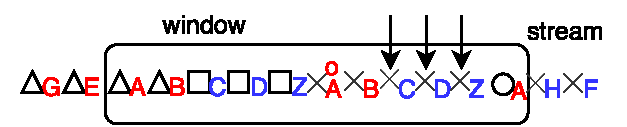
\includegraphics[width=5in]{img/3-siqre.pdf}
    \caption{Query Relevance Example}
    \label{fig:3-siqre}
\end{figure}

The system can be totally blind or literate about streaming data query relevance, depending on whether or not a query relevance query/ontology is deployed, as well as how comprehensive the knowledge of the streaming data is encoded. 
For example, in Figure \ref{fig:3-siqre}, $\largesquare_{D}$ is irrelevant as a defender can never commit an offside offence. 
If such knowledge is also included in the query relevance ontology, the query relevance ontology becomes more comprehensive, and more irrelevant data can be filtered out. 
As the consequences of the query relevance ontology, data items pointed by arrows are not relevant to the current query and thus can be filtered out of the window.


There are several general principles in order to prepare query relevance ontologies.
First, to understand the target and requirements of the use case. 
Since query relevance ontology is domain-specific, and is possibly dependent on the background ontology, understanding what is expected out of the use case can provide a clear ontology construction goal. 
Second, to understand the data, meaning to know what data is useful or useless to the use case.
The patterns of relevant data will then be composed and encoded in the ontology.
Third, keep in mind that query relevance ontology will not work for different queries, since it is so customized to one query in one use case.
%
\section{Comparison Rule}
The semantic importance model encodes the aspects to provide a multi dimensional view on importance.
For example, $[\tau_{e}, \tau_{a}]$ uses expiration timestamp ($\tau_{e}$) and arrival timestamp ($\tau_{a}$) to describe data importance; while $[t^{tm}_{s}, f_{qp}]$ uses trustworthiness and query participation frequency to describe data importance. 
However, in order to enable order-awareness, there should be a comparable rule to be used to rank the data according to its importance. 
This rule, named semantic importance comparison rule, evaluates the data importance by comparing all dimensions of a priority vector for each data item. 
The comparison rule uses comparable operator ``$<$'', ``$>$'' and ``$==$'' to compare priority vector elements. 
The semantics of these comparable operators are defined in Table \ref{tab:cos}.

\begin{table*}[!htbp]
	\centering
	\caption{Comparable Operator Semantics}
	\label{tab:cos}
	\begin{tabular}{|c|c|c|c|} \hline
		SI & $<$ & $>$ & $==$ \\ \hline
        $\tau_{g}$ & \makecell{if $\tau^{1}_{g}$ is before than $\tau^{2}_{g}$ \\ $\Rightarrow \tau^{1}_{g} < \tau^{2}_{g}$} & \makecell{if $\tau^{1}_{g}$ is after than $\tau^{2}_{g}$ \\ $\Rightarrow \tau^{1}_{g} > \tau^{2}_{g}$} & \makecell{$\tau^{1}_{g}$ is equal to $\tau^{2}_{g}$ \\ $\Rightarrow \tau^{1}_{g} == \tau^{2}_{g}$} \\ \hhline{|=#=|=|=|}
		$\tau_{a}$ & \makecell{if $\tau^{1}_{a}$ is before than $\tau^{2}_{a}$ \\ $\Rightarrow \tau^{1}_{a} < \tau^{2}_{a}$} & \makecell{if $\tau^{1}_{a}$ is after than $\tau^{2}_{a}$ \\$\Rightarrow \tau^{1}_{a} > \tau^{2}_{a}$} & \makecell{if $\tau^{1}_{a}$ is equal to $\tau^{2}_{a}$ \\$\Rightarrow \tau^{1}_{a} == \tau^{2}_{a}$} \\ \hline
		$\tau_{e}$ & \makecell{if $\tau^{1}_{e}$ is before than $\tau^{sys}$ \\ if $\tau^{2}_{e}$ is before than $\tau^{sys}$ \\$\Rightarrow \tau^{1}_{e} < \tau^{2}_{e}$}& \makecell{if $\tau^{1}_{e}$ is after than $\tau^{sys}$ \\ if $\tau^{2}_{e}$ is before than $\tau^{sys}$\\$\Rightarrow \tau^{1}_{e} > \tau^{2}_{e}$} & \makecell{if $\tau^{1}_{e}$ is before than $\tau^{sys}$ \\ if $\tau^{2}_{e}$ is before than $\tau^{sys}$ \\ $\Rightarrow \tau^{1}_{e} == \tau^{2}_{e}$ \\if $\tau^{1}_{e}$ is after than $\tau^{sys}$\\if $\tau^{2}_{e}$ is after than $\tau^{sys}$\\$\Rightarrow \tau^{1}_{e} == \tau^{2}_{e}$} \\ \hline
        $\tau_{qp}$ & \makecell{if $\tau^{1}_{qp}$ is before than $\tau^{2}_{qp}$\\ $\Rightarrow \tau^{1}_{qp} < \tau^{2}_{qp}$} & \makecell{if $\tau^{1}_{qp}$ is after than $\tau^{2}_{qp}$ \\ $\Rightarrow \tau^{1}_{qp} > \tau^{2}_{qp}$} & \makecell{if $\tau^{1}_{qp}$ is equal to $\tau^{2}_{qp}$ \\ $\Rightarrow \tau^{1}_{qp} == \tau^{2}_{qp}$} \\ \hline
        $f_{qp}$ & $f^{1}_{qp} < f^{2}_{qp}$ & $f^{1}_{qp} > f^{2}_{qp}$ & $f^{1}_{qp} == f^{2}_{qp}$ \\ \hline
        $qrf$ & false $<$ true & true $>$ false & \makecell{true == true \\false == false} \\ \hline
        $t^{tm}_{s}$ & $t^{tm}_{s1} < t^{tm}_{s2}$ & $t^{tm}_{s1} > t^{tm}_{s2}$ & $t^{tm}_{s1} == t^{tm}_{s2}$ \\ \hline        
	\end{tabular}
\end{table*}

In Table \ref{tab:cos}, $\tau$ represents timestamps, $\tau^{sys}$ denotes current system time, $t^{tm}_{s}$ refers to trust score by a trust model $tm$, $qrf$ represents query relevance filter. 
When query relevance is included in the importance description, a data filtering SPARQL query will be executed. 

When comparing priority vectors\footnote{Only priority vectors with same amount of elements can be compared.}, the leftmost element will be compared first. 
If there is a tie for this element, the second element then will be compared, and so on. 
This is because the priority vector requires its elements to be ordered according to a preference function, as a consequence, the more preferred elements are placed on more lefter side. 
For example, if a data item is associated with an explicit expiration timestamp ($\tau_{e}$), the priority vector $[\tau_{e}]$ will consider unexpired data to be important.
If the data frequency of the query participation ($f_{qp}$) is included, the priority vector $[\tau_{e}, f_{qp}]$ emphasizes $\tau_{e}$ over $f_{qp}$ to guarantee that one unexpired data item is more important than another.
For all unexpired data, what is more important is which participates more frequently in the query.
Expired data becomes less important no matter how frequent its query participation is.
By explicitly characterizing the importance for each data item in the stream, order-awareness can be realized by ranking the semantic importance priority vectors via the following algorithm:

\begin{algorithm}[!htbp]
  priority vectors $v_{1} = [x_{1}, ... , x_{n}]$, $v_{2} = [y_{1}, ... , y_{n}]$ \;
  int i = 0 \;
  \While{$i < n$} {
	  \uIf{$x_{i} > y_{i}$}{
    	return $v_{1} > v_{2}$ \;
  	  }
	  \uElseIf{$x_{i} < y_{i}$}{
    	return $v_{1} < v_{2}$ \;
 	  }
  	  \uElse{
    	i++ \;
  	  } 	
  }
  \uIf{i == n} { 
  	return $v_{1} == v_{2}$ \;  
  }
\caption{Semantic Importance Comparison Algorithm}
\end{algorithm}
%
\section{Window Management Strategies}
A sliding window is defined as a finite subset of the stream \cite{botan2010secret}. 
It has two parameters, a window size (width) that determines how much data a window can contain; 
a window step (slide) that is the distance between two consecutive windows. 
A window has different types \cite{barbieri2010querying}, \cite{patroumpas2006window}.
For all details about windows and operational semantics, please refer to Chapter 2. 

As mentioned in the Introduction Section, the silent logical assumption that older information becomes irrelevant at some point \cite{barbieri2010stream}, \cite{stuckenschmidt2010towards} is very popular in stream reasoning \cite{golab2003processing}, \cite{barbieri2010deductive}.
Based on this silent logical assumption, the dominant window management strategy is first in first out (FIFO). 
This strategy consumes the most recent data based on the window step. 
In order to guarantee identical window size during processing, the amount of data to be evicted should be strictly identical with that of data to be consumed.
The data to be evicted is usually the oldest.

In order to illustrate how semantic importance enabled window management strategies can manage the data items in the window, we will use a running example with a physical sliding window of a size of four tuples, and a step of one tuple. 
Six strategies, including FIFO, will be shown in detail about the way and differences they manage streaming data in the window.

\textbf{FIFO}:
First In First Out (FIFO) describes data importance with a single arrival timestamp ($\tau_{a}$) from the logical provenance aspect. 
Its priority vector is $[\tau_{a}]$.

\begin{figure}[!htbp]
	\centering
    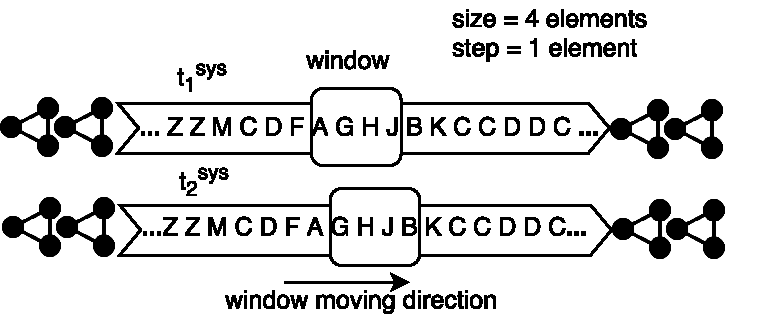
\includegraphics[width=5in]{img/3-sififo.pdf}
    \caption{FIFO Management Strategy}
    \label{fig:3-sififo}
\end{figure}

In Figure \ref{fig:3-sififo}, data \textbf{arrives} in a logical order such that $\tau^{A}_{a} < \tau^{G}_{a} < \tau^{H}_{a} < \tau^{J}_{a} < \tau^{B}_{a}$.
At $t^{sys}_{1}$, items A, G, H, and J are in the window. 
At $t^{sys}_{2}$, as window proceeds, A is evicted so as to consume B. 
Given the arrival order, the data rankings at $t^{sys}_{1}$ and $t^{sys}_{2}$ are shown in Table \ref{tab:fifo}.
Data gets re-ranked as window moves, and data ranked at the bottom will be evicted.

\begin{table}[!htbp]
\centering
\caption{Data Ranking Under FIFO}
\label{tab:fifo}
\begin{tabular}{|c|c|c||c|c|c|}
\hline
\multicolumn{3}{|c||}{$t^{sys}_{1}$} & \multicolumn{3}{c|}{$t^{sys}_{2}$} \\ \hhline{|===#===|}
rank & data & $\tau_{a}$ & rank & data & $\tau_{a}$ \\ \hhline{|=|=|=#=|=|=|}
1 & J & $\tau^{J}_{a}$ & 1 & B & $\tau^{B}_{a}$ \\ \hline
2 & H & $\tau^{H}_{a}$ & 2 & J & $\tau^{J}_{a}$ \\ \hline
3 & G & $\tau^{G}_{a}$ & 3 & H & $\tau^{H}_{a}$ \\ \hline
4 & A & $\tau^{A}_{a}$ & 4 & G & $\tau^{G}_{a}$ \\ \hline
\end{tabular}
\end{table}

\textbf{FEFO}:
First Expired First Out (FEFO) describes data importance with a single expiration timestamp ($\tau_{e}$) from the logical provenance aspect. 
Its priority vector is $[\tau_{e}]$.

\begin{figure}[!htbp]
	\centering
    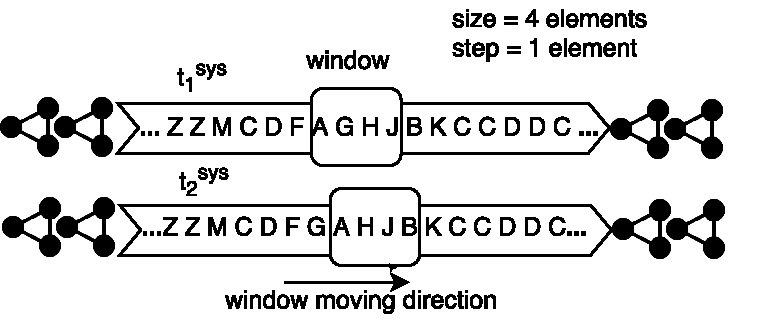
\includegraphics[width=5in]{img/3-sifefo.pdf}
    \caption{FEFO Management Strategy}
    \label{fig:3-sifefo}
\end{figure}

In Figure \ref{fig:3-sifefo}, at $t^{sys}_{1}$, data \textbf{arrives} in a logical order such that $\tau^{A}_{a} < \tau^{G}_{a} < \tau^{H}_{a} < \tau^{J}_{a} < \tau^{B}_{a}$, \textbf{expires}\footnote{We use the ``$==$'' semantics from Table \ref{tab:cos}. Note that the value of $\tau^{A}_{e}$, $\tau^{J}_{e}$ and $\tau^{H}_{e}$ are not necessarily numerically equal.} in a logical order such that $\tau^{G}_{e} < t^{sys}_{1} < \tau^{B}_{e} < t^{sys}_{2} < \tau^{A}_{e} == \tau^{J}_{e} == \tau^{H}_{e}$.
At $t^{sys}_{1}$, items A, G, H, and J are in the window, G is expired.
At $t^{sys}_{2}$, G is evicted to consume B, which will be evicted next. 
Note that even though G arrives later than A, G is evicted because of FEFO management strategy,
and even though B is the latest data item, it is also an expired data item, thus needs to be evicted. 
Data rankings at $t^{sys}_{1}$ and $t^{sys}_{2}$ are listed in Table \ref{tab:fefo}. 
The data item ranks at the bottom will be evicted. 

\begin{table}[!htbp]
\centering
\caption{Data Ranking Under FEFO}
\label{tab:fefo}
\begin{tabular}{|c|c|c||c|c|c|}
\hline
\multicolumn{3}{|c||}{$t^{sys}_{1}$} & \multicolumn{3}{c|}{$t^{sys}_{2}$} \\ \hhline{|===#===|}
rank & data & $\tau_{e}$ & rank & data & $\tau_{e}$ \\ \hhline{|=|=|=#=|=|=|}
1 & H, J, A & $\tau^{H}_{e}$, $\tau^{J}_{e}$, $\tau^{A}_{e}$ & 1 & H, J, A & $\tau^{H}_{e}$, $\tau^{J}_{e}$, $\tau^{A}_{e}$ \\ \hline
2 & G & $\tau^{G}_{e}$ & 2 & B & $\tau^{B}_{e}$ \\ \hline
\end{tabular}
\end{table}

\textbf{LFU}:
Least Frequently Used (LFU) is a classic caching algorithm \cite{crp2018}, but not commonly used in the window management.
LFU describes the data importance with a single query participation frequency ($f_{qp}$) from the query participation aspect. 
Its priority vector is $[f_{qp}]$.

\begin{figure}[!htbp]
	\centering
    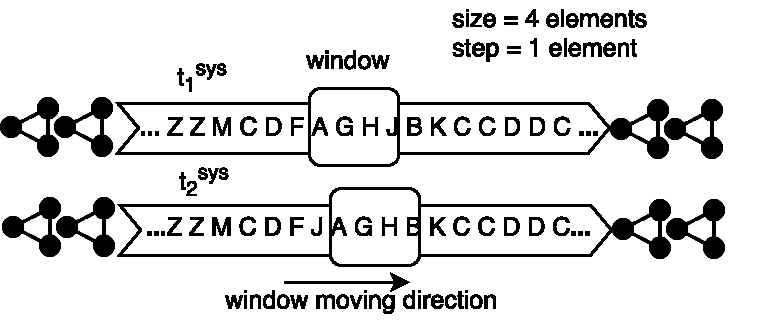
\includegraphics[width=5in]{img/3-silfu.pdf}
    \caption{LFU Management Strategy}
    \label{fig:3-silfu}
\end{figure}

In Figure \ref{fig:3-silfu}, data \textbf{arrives} in a logical order such that $\tau^{A}_{a} < \tau^{G}_{a} < \tau^{H}_{a} < \tau^{J}_{a} < \tau^{B}_{a}$. 
As soon as the data arrives in the window, its $f_{qp}$ is initialized to be 0.
$f^{X}_{qp}$ will increase by 1 if the data item X participates in the query once.
At $t^{sys}_{1}$, assuming that $f^{A}_{qp} = 3$, $f^{G}_{qp} = 2$, $f^{H}_{qp} = 0$, $f^{J}_{qp} = 0$. 
Since $t^{H}_{qp} = t^{J}_{qp} = 0$, both H and J rank at the bottom in Table \ref{tab:lfu}. 
Either H or J will be evicted in an undecided way because of the window step is 1 tuple. 
In Figure \ref{fig:3-silfu}, let's tentatively evict J to consume B. 
After query is executed, assuming that B participates in the query thus $f^{B}_{qp}$ becomes 1.
Then, data items in the window get re-ranked at $t^{sys}_{2}$.
Since $f^{H}_{qp}$ is 0 and the smallest, data item H will be ranked at the bottom and evicted next. 

\begin{table}[!htbp]
\centering
\caption{Data Ranking Under LFU}
\label{tab:lfu}
\begin{tabular}{|c|c|c||c|c|c|}
\hline
\multicolumn{3}{|c||}{$t^{sys}_{1}$} & \multicolumn{3}{c|}{$t^{sys}_{2}$} \\ \hhline{|===#===|}
rank & data & $f_{qp}$ & rank & data & $f_{qp}$ \\ \hhline{|=|=|=#=|=|=|}
1 & A & 3 & 1 & A & 4 \\ \hline
2 & G & 2 & 2 & G & 3 \\ \hline
3 & H, J & 0 & 3 & B & 1 \\ \hline
4 & - & - & 4 & H & 0 \\ \hline
\end{tabular}
\end{table}

\textbf{FE-LFU-FO}:
First Expired Least Frequently Used First Out (FE-LFU-FO) is a more complex window management strategy. 
It describes the data importance with the expiration timestamp ($\tau_{e}$) and the query participation frequency ($f_{qp}$).
Its priority vector is $[\tau_{e}, f_{qp}]$, which emphasizes $\tau_{e}$ over $f_{qp}$. 

\begin{figure}[!htbp]
	\centering
    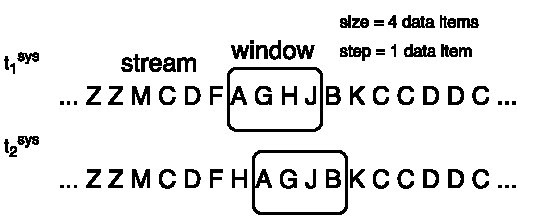
\includegraphics[width=5in]{img/3-sifelfufo.pdf}
    \caption{FE-LFU-FO Management Strategy}
    \label{fig:3-sifelfufo}
\end{figure}

In Figure \ref{fig:3-sifelfufo}, assuming that data arrives in a logical order such that $\tau^{A}_{a} < \tau^{G}_{a} < \tau^{H}_{a} < \tau^{J}_{a} < \tau^{B}_{a}$, and expires in an order such that $\tau^{H}_{e} < t^{sys}_{1} < t^{sys}_{2} < \tau^{G}_{e} == \tau^{J}_{e} == \tau^{A}_{e} == \tau^{B}_{e}$.
At $t^{sys}_{1}$, we can compare data items priority vector according to the comparison rule. 
Since $[\tau^{H}_{e}, 4] < [t^{sys}_{1}, -] < [\tau^{G}_{e}, 0] < [\tau^{J}_{e}, 2] < [\tau^{A}_{e}, 3]$, H ranks at the bottom thus evicted even though it participated most in the query. 
At $t^{sys}_{2}$, $[t^{sys}_{2}, -] < [\tau^{G}_{e}, 0] == [\tau^{B}_{e}, 0] < [\tau^{J}_{e}, 3] < [\tau^{A}_{e}, 4]$.
Table \ref{tab:felfufo} shows the data rankings. 
At $t^{sys}_{2}$, both B and G are ranked at the bottom, thus either will be evicted due to the window step. 

\begin{table}[!htbp]
\centering
\caption{Data Ranking Under FE-LFU-FO}
\label{tab:felfufo}
\begin{tabular}{|c|c|c|c||c|c|c|c|}
\hline
\multicolumn{4}{|c||}{$t^{sys}_{1}$} & \multicolumn{4}{c|}{$t^{sys}_{2}$} \\ \hhline{|====#====|}
rank & data & $\tau_{e}$ & $f_{qp}$ & rank & data & $\tau_{e}$ & $f_{qp}$ \\ \hhline{|=|=|=|=#=|=|=|=|}
1 & A & $\tau^{A}_{e}$ & 3 & 1 & A & $\tau^{A}_{e}$ & 4 \\ \hline
2 & J & $\tau^{J}_{e}$ & 2 & 2 & J & $\tau^{J}_{e}$ & 3 \\ \hline
3 & G & $\tau^{G}_{e}$ & 0 & 3 & B,G & $\tau^{B}_{e}$, $\tau^{G}_{e}$ & 0 \\ \hline
4 & H & $\tau^{H}_{e}$ & 4 & 4 & - & - & - \\ \hline
\end{tabular}
\end{table}

\textbf{LFU-FE-FO}:
Least Frequently Used First Expired First Out (LFU-FE-FO), just like FE-LFU-FO, describes the data importance with $\tau_{e}$ and $f_{qp}$. 
Its priority vector $[f_{qp}, \tau_{e}]$, albeit has the same elements as FE-LFU-FO's $[\tau_{e}, f_{qp}]$, it ranks data items in a totally different way. 

\begin{figure}[!htbp]
	\centering
    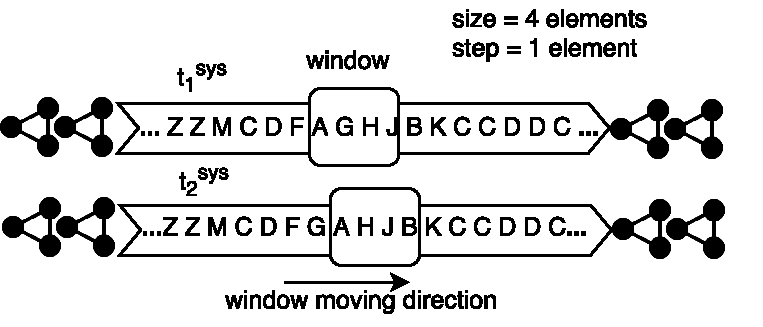
\includegraphics[width=5in]{img/3-silfufefo.pdf}
    \caption{LFU-FE-FO Management Strategy}
    \label{fig:3-silfufefo}
\end{figure}

In Figure \ref{fig:3-silfufefo}, assuming that data arrives in a logical order such that $\tau^{A}_{a} < \tau^{G}_{a} < \tau^{H}_{a} < \tau^{J}_{a} < \tau^{B}_{a}$, and expires in a logical order such that $\tau^{H}_{e} < t^{sys}_{1} < t^{sys}_{2} < \tau^{G}_{e} == \tau^{J}_{e} == \tau^{A}_{e} == \tau^{B}_{e}$. 
Together with Table \ref{tab:lfufefo}, at $t^{sys}_{1}$, $[-, t^{sys}_{1}] < [0, \tau^{G}_{e}] < [2, \tau^{J}_{e}] < [3, \tau^{A}_{e}] < [4, \tau^{H}_{e}]$. 
G is ranked at the bottom thus will be evicted.
However, H is ranked at the top even though H is expired. 
What is even worse is that H has the most query participation frequency, that almost guarantees that H will be at the top forever, resulting in invalid answers.
At $t^{sys}_{2}$, $[-, t^{sys}_{2}] < [0, \tau^{B}_{e}] < [3, \tau^{J}_{e}] < [4, \tau^{A}_{e}] < [5, \tau^{H}_{e}]$.
H, A and J's query participation frequencies increase by 1, while B doesn't participate in the query.
Thus B is ranked at the bottom and will be evicted. 

From this example, we can see that even though the window management strategies formed by combining different semantic importance aspects can be various, what's crucial behind it is to careful design the combination so that the strategy can manage data in a legit way. 

\begin{table}[!htbp]
\centering
\caption{Data Ranking Under LFU-FE-FO}
\label{tab:lfufefo}
\begin{tabular}{|c|c|c|c||c|c|c|c|}
\hline
\multicolumn{4}{|c||}{$t^{sys}_{1}$} & \multicolumn{4}{c|}{$t^{sys}_{2}$} \\ \hhline{|====#====|}
rank & data & $f_{qp}$ & $\tau_{e}$ & rank & data & $f_{qp}$ & $\tau_{e}$ \\ \hhline{|=|=|=|=#=|=|=|=|}
1 & H & 4 & $\tau^{H}_{e}$ & 1 & H & 5 & $\tau^{H}_{e}$ \\ \hline
2 & A & 3 & $\tau^{A}_{e}$ & 2 & A & 4 & $\tau^{A}_{e}$ \\ \hline
3 & J & 2 & $\tau^{J}_{e}$ & 3 & J & 3 & $\tau^{J}_{e}$ \\ \hline
4 & G & 0 & $\tau^{G}_{e}$ & 4 & B & 0 & $\tau^{B}_{e}$ \\ \hline
\end{tabular}
\end{table}

\textbf{FE-LFU-FI-FO}:
First Expired Least Frequently Used First In First Out (FE-LFU-FI-FO) uses the expiration timestamp ($\tau_{e}$), query participation frequency ($f_{qp}$) and arrival timestamp ($\tau_{a}$) to describe the data importance.
Its priority vector is $[\tau_{e}, f_{qp}, \tau_{a}]$, which contains three elements.

\begin{figure}[!htbp]
	\centering
    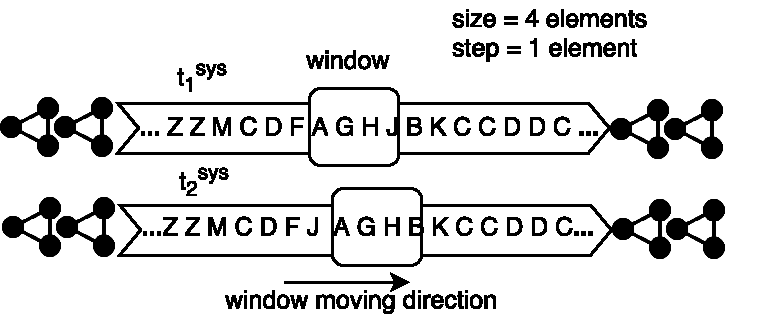
\includegraphics[width=5in]{img/3-sifelfufifo.pdf}
    \caption{FE-LFU-FI-FO Management Strategy}
    \label{fig:3-sifelfufifo}
\end{figure}

In Figure \ref{fig:3-sifelfufifo}, assuming that data arrives in a logical order such that $\tau^{A}_{a} < \tau^{G}_{a} < \tau^{H}_{a} < \tau^{J}_{a} < \tau^{B}_{a}$, and expires in a logical order such that  $\tau^{J}_{e} < t^{sys}_{1} < \tau^{G}_{e} < t^{sys}_{2} < \tau^{H}_{e} == \tau^{A}_{e} == \tau^{B}_{e}$.
At $t^{sys}_{1}$, $[\tau^{J}_{e}, 6, \tau^{J}_{a}] < [t^{sys}_{1}, -, -] < [\tau^{G}_{e}, 0, \tau^{G}_{a}] < [\tau^{H}_{e}, 1, \tau^{H}_{a}] < [\tau^{A}_{e}, 4, \tau^{A}_{a}]$. 
At $t^{sys}_{2}$, $[\tau^{G}_{e}, 0, \tau^{J}_{a}] < [t^{sys}_{2}, -, -] < [\tau^{B}_{e}, 0, \tau^{B}_{a}] < [\tau^{H}_{e}, 2, \tau^{H}_{a}] < [\tau^{A}_{e}, 5, \tau^{A}_{a}]$. 
With these orderings, data is ranked as in Table \ref{tab:felfufifo}. 
Data ranked at the bottom will be evicted. 

\begin{table}[!htbp]
\centering
\caption{Data Ranking Under FE-LFU-FI-FO}
\label{tab:felfufifo}
\begin{tabular}{|c|c|c|c|c||c|c|c|c|c|}
\hline
\multicolumn{5}{|c||}{$t^{sys}_{1}$} & \multicolumn{5}{c|}{$t^{sys}_{2}$} \\ \hhline{|=====#=====|}
rank & data & $\tau_{e}$ & $f_{qp}$ & $\tau_{a}$ & rank & data & $\tau_{e}$ & $f_{qp}$ & $\tau_{a}$ \\ \hhline{|=|=|=|=|=#=|=|=|=|=|}
1 & A & $\tau^{A}_{e}$ & 4 & $\tau^{A}_{a}$ & 1 & A & $\tau^{A}_{e}$ & 5 & $\tau^{A}_{a}$ \\ \hline
2 & H & $\tau^{H}_{e}$ & 1 & $\tau^{H}_{a}$ & 2 & H & $\tau^{H}_{e}$ & 2 & $\tau^{H}_{a}$ \\ \hline
3 & G & $\tau^{G}_{e}$ & 0 & $\tau^{G}_{a}$ & 3 & B & $\tau^{B}_{e}$ & 0 & $\tau^{A}_{a}$ \\ \hline
4 & J & $\tau^{J}_{e}$ & 6 & $\tau^{J}_{a}$ & 4 & G & $\tau^{G}_{e}$ & 0 & $\tau^{G}_{a}$ \\ \hline
\end{tabular}
\end{table}

The above six strategies are certainly not an exhaustive list of all the window management strategies that semantic importance can enable. 
The point is provide both examples and evidence that semantic importance can not only enable classic FIFO strategy, but also smarter and more flexible strategies. 
FE-LFU-FO and LFU-FE-FO strategies manage data differently even though their priority vectors have same elements. 
Other possible strategies with priority vectors such as $[t^{tm1}_{s}, \tau_{e}, \tau_{a}]$, $[qrf, t^{tm1}_{s}, t^{tm2}_{s}, \tau_{e}, \tau_{a}]$ are also very similar to implement.
%
\section{Window Semantics}
Semantic importance is an interesting idea to pursuit because it brings a better concept of what to forget, so as to shrink the window size during processing the gigantic data streams.
However, forgetting based on FIFO is only logical.
The silent logical assumption is probably a good reflection of logically-oriented-only importance.
The soccer example shows that the ``importance'' is a deeper notion, a more domain specific notion, which cannot be adequately modeled merely by time alone. 
One motivation of this dissertation is to take the notion of importance into semantics by bringing the domain into the computation with an efficient way. 
This requires not only to model the importance of the data, but also to extend the current sliding window semantics that is related to the silent logical assumption. 

What will be shown later illustrates why it is important to extend the window semantics in order to realize the flexible and smart window management strategies.
The method is to re-define the window size and step, as well as to extend the sliding logical window semantics with the lower-bounded landmark window whose lower bound is fixed permanently, and upper bound proceeds. 
This extended window semantics can work well with the semantic importance. 
%
\subsection{Problems in Existing Window Semantics}
``\textbf{A window W over a stream S is a finite subset of S}'' \cite{dindar2013modeling}.
A sliding window has two parameters, size and step, both have been mentioned and defined in related work \cite{beck2015lars}, \cite{dindar2013modeling}, \cite{prud2008sparql}, \cite{botan2010secret}, \cite{arasu2006cql}.
\cite{dindar2013modeling} requires that all windows defined over a stream must have the same size and step, with a restriction that the step could be any value that must be no bigger than the size.
\cite{patroumpas2006window} indicates that physical window step is 1 with the statement that ``... window states are determined only at single-tuple units ...". 
\cite{calbimonte2010enabling} mentions that ``... if the step is larger than the range then the windows sample the stream ...", indicating that the step can be larger than the size. 
As you can see, there are already some differences on how researchers understand and define window semantics. 
Window semantics is important to define a window and managing data.

In this section, I argue that none of the existing window semantics can be adapted when equipping window with management strategies other than FIFO.  
As a result, existing window semantics need to be extended. 

\begin{figure}[!htbp]
	\centering
    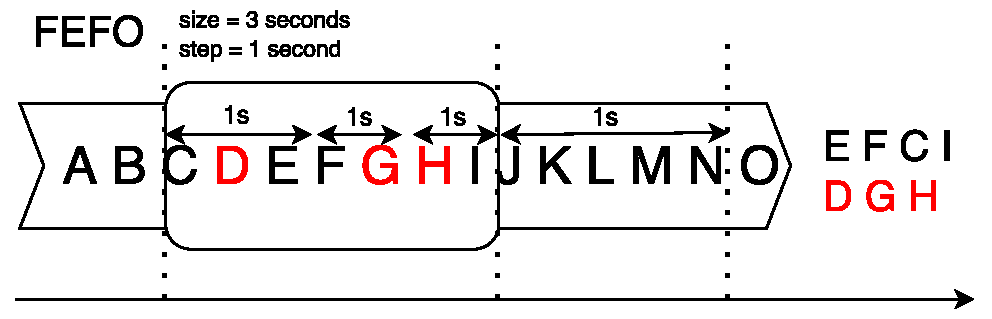
\includegraphics[width=5in]{img/3-wsti.pdf}
    \caption{Logical Sliding Window Under FEFO}
    \label{fig:3-wsti}
\end{figure}

Consider the example in Figure \ref{fig:3-wsti}, which is a logical sliding window under FEFO management strategy, with a size of 3 seconds and a step of 1 second. 
Assume that data items D, G, and H are expired (marked in red), thus ranked at the bottom. 
At this point, window size is still 3 seconds as $t^{I}_{a} - t^{C}_{a} = 3s$, even if D, G, and H are evicted.  
As a consequence, the sliding window will not move as it is still full according to its semantics, so that the continuous processing will be halted. 

\begin{figure}[!htbp]
	\centering
    
\includegraphics[width=5in]{img/3-wstu.pdf}
    \caption{Physical Sliding Window Under FEFO}
    \label{fig:3-wstu}
\end{figure}

In Figure \ref{fig:3-wstu}, a physical (tuple-based) sliding window manages data under FEFO. 
At this moment, data items G and H are expired (marked in red), thus ranked at the bottom. 
However, since the current window semantics defines its step to be 1 and fixed, it can only evict one data item. 
No matter which data item is evicted, a worse case is that the kept expired data item participated in the query, causing the early expiration problem and resulting invalid query answers. 

The two problems above have shown that existing window semantics cannot work well with semantic importance enabled window management strategies. 
The primary reason is that these strategies manage data in a ``data item'' granularity, rather than a simple ``logical'' granularity. 
%
\subsection{Extended Logical Window Semantics}
This dissertation will use the definitions of lower bound ($\tau_{l}$), upper bound ($\tau_{u}$), data stream ($S$), current stream contents ($S(\tau)$), current stream instance ($s_{\tau}$), time domain ($T$) and lower-bounded landmark window ($W^{lbl}$) from \cite{patroumpas2006window}.
A logical lower-bounded landmark window ($W^{lbl}_{\tau}$) is employed as an extended window for a logical sliding window.
For $W^{lbl}_{\tau}$, its $\tau_{l}$ is fixed permanently, while $\tau_{u}$ proceeds as time goes by. 
Figure \ref{fig:3-lw} shows an example of $W^{lbl}_{\tau}$. 

\begin{figure}[!htbp]
	\centering
    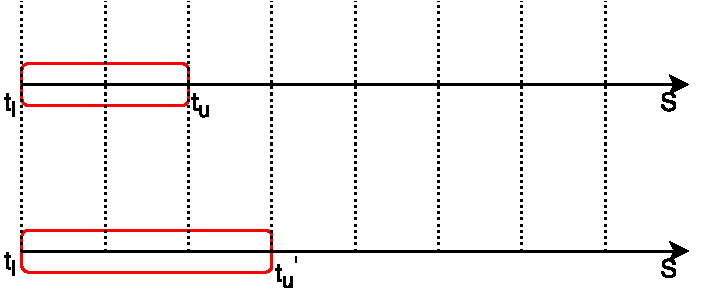
\includegraphics[width=5in]{img/3-lw.pdf}
    \caption{Logical Lower-bounded Landmark Window Example}
    \label{fig:3-lw}
\end{figure}

Rather than defining window size, this dissertation uses the definition from \cite{tangwongsan2015general}:
\textbf{``the instantaneous window size ($n_{\tau}$) at time $\tau$ is defined as the number of tuples in the current active window.''}
With this definition, $W^{lbl}_{\tau}$ window size can vary. 
We define a logical window step for $W^{lbl}_{\tau}$: 
\textbf{window step ($n_{\beta}$) is defined as the number of tuples within next $\beta$ measurement units  \cite{patroumpas2006window} (such as seconds, minutes, etc)}. 

\begin{figure}[!htbp]
	\centering
    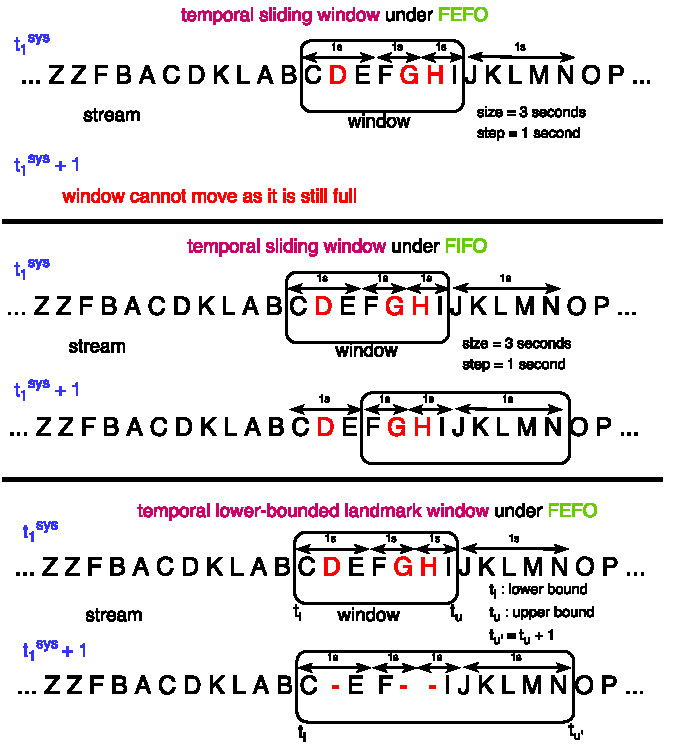
\includegraphics[width=5in]{img/3-psewsti.pdf}
    \caption{Extended Logical Window Semantics Example}
    \label{fig:3-psewsti}
\end{figure}

Figure \ref{fig:3-psewsti} shows how the extended logical window semantics can work with semantic importance enabled window management strategies (such as FEFO) when managing data streams. 
By leveraging the extended logical window semantics from the landmark window, the logical lower-bounded landmark window can continue to proceed after evicting all the expired data.
This is much flexible than a logical sliding window that will have to remove the oldest data under FIFO in order to proceed, which results in removing data items that are still valid (such as C and E in Figure \ref{fig:3-wsti}), and keeping data items that are expired (such as G and H in Figure \ref{fig:3-wsti}). 

\begin{table}[!htbp]
	\centering
	\caption{Window Semantics Example}
	\label{tab:lwsw}
	\begin{tabular}{|c||c|c|}
	\hline
	& \makecell{landmark window \\ under FEFO} & \makecell{sliding window \\ under FIFO} \\ \hhline{|=#=|=|}
	\makecell{window size} & \makecell{$n_{t_{u}} = 7$\\ $n_{t_{u'}} = 9$} & \makecell{2s (7 tuples)\\ 2s (9 tuples)} \\ \hline
	\makecell{query: do both C and N exist \\ in the stream? (early eviction) \\ ground truth: yes } & answer: yes  & answer: no \\ \hline
	\makecell{query: do both G and N exist \\ in the stream? (early expiration) \\ ground truth: no} & answer: no & answer: yes \\ \hline
	\end{tabular}
\end{table}

Table \ref{tab:lwsw} shows the different results of different window semantics. 
We have used the physical window size definition for the landmark window. 
At $t_{u}$ and $t_{u'}$ time in Figure \ref{fig:3-psewsti}, its size is 7 and 9 respectively. 
For the sliding window under FIFO, its size is logical, which is 2 seconds. 
At $t_{1}^{sys}$ and $t_{1}^{sys} + 1$ time in Figure \ref{fig:3-psewsti}, the number of tuples in the sliding window is 7 and 9 respectively.
Thus, even though the landmark window seems to have ``infinite'' growth as its lower bound fixed permanently and its upper bound proceeds, the number of tuples in the window does not necessarily become ``infinite'', thanks to the extended window size definition. 
In this example, the span of the landmark window is 4 seconds, which is larger than the sliding window size of 2 seconds, but the number of tuples in both windows is equal.

The landmark window semantics can also help solve the early eviction and early expiration problem. 
The query ``do both C and N exist in the stream'' will have a false-negative answer from the sliding window under FIFO, as C has to be evicted in order to get N. 
This is an early eviction problem.
In a landmark window with FEFO, C stays as it is not expired, thus can provide the correct answer. 
For the query ``do both G and N exist in the stream'', a false-positive answer will be given by the sliding window under FIFO, as G is expired within the window but cannot be evicted. 
This is an early expiration problem.
The landmark window with FEFO strategy can provide correct result as all the expired data can be evicted without affecting the continuous data consumption and processing.  
%
\subsection{Extended Physical Window Semantics}
Different from the logical window, this dissertation will use a sliding physical (tuple-based) window ($W_{\#}$).
From the window size definition \cite{tangwongsan2015general}, a sliding physical window size $n_{\tau}$ is always a fixed value.
The only part to be extended from the sliding physical window semantics is the step. 
\textbf{The step ($n_{\beta}$) is defined as a variable with its range as ${n_{\beta} = \{\ n_{\beta} \ |\ 0 \leq n_{\beta} \leq n_{\tau}}\}$.}

\begin{figure}[!htbp]
	\centering
    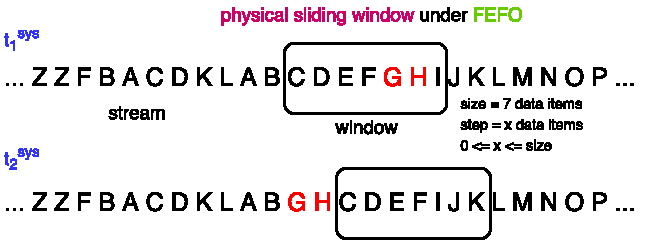
\includegraphics[width=5in]{img/3-psewstu.pdf}
    \caption{Extended Physical Window Semantics Under FEFO}
    \label{fig:3-psewstu}
\end{figure}

Figure \ref{fig:3-psewstu} shows how data can be managed with FEFO, and the extended physical window semantics. 
Since the window step is now a variable no bigger than the window size, evicting data becomes much more flexible: if two data items are expired, both of them will be evicted. 
Thus the window can continue to consume next two new data items. 
If all of the data are expired in the window, then evict all of them to consume next $n_{\tau}$ data items. 
This flexible window step guarantees that all of the unimportant data items are evicted, so as to solve the problems such as the early expiration. 
One thing to note is that, with FEFO, data has to be expired to be evicted.
If all of the data are not expired, the window will not proceed but wait till at least one of them is expired. 
This indicates that the window management strategies manage data differently, and it is crucial to choose a proper strategy to keep the desired data for query.
%
\subsection{Discussion}
\begin{table}[!htbp]
\centering
\caption{Window Semantics Comparison}
\label{tab:wsc}
\begin{tabular}{|c||c|c|}
\hline
 & \begin{tabular}[c]{@{}c@{}}Sliding Window \\ Semantics\end{tabular} & \begin{tabular}[c]{@{}c@{}}Extended Window \\ Semantics\end{tabular} \\ \hhline{|=#=|=|}
\begin{tabular}[c]{@{}c@{}}logical \\ window ($W_{\tau}$)\end{tabular} & sliding window & \begin{tabular}[c]{@{}c@{}}lower-bounded \\ landmark window\end{tabular} \\ \hline
$W_{\tau}$ size & \begin{tabular}[c]{@{}c@{}}fixed.\\ defined with logical \\ measurement units (e.g. 2s)\end{tabular} & \begin{tabular}[c]{@{}c@{}}can vary.\\ defined as $n_{\tau}$, number \\ of tuples at an instantaneous \\ time-point (e.g. 23)\end{tabular} \\ \hline
$W_{\tau}$ step & \begin{tabular}[c]{@{}c@{}}fixed.\\ defined with logical\\  measurement units (e.g. 1s)\end{tabular} & \begin{tabular}[c]{@{}c@{}}fixed.\\ defined as $n_{\beta}$, number \\ of tuples within next $\beta$ \\ measurement units.(e.g. 15)\end{tabular} \\ \hhline{|=#=|=|}
\begin{tabular}[c]{@{}c@{}}physical\\window ($W_{\#}$)\end{tabular} & sliding window & sliding window \\ \hline
$W_{\#}$ size & \begin{tabular}[c]{@{}c@{}}fixed.\\ defined as $n_{\tau}$, number \\ of tuples at an instantaneous \\ time-point (e.g. 23)\end{tabular} & \begin{tabular}[c]{@{}c@{}}fixed.\\ defined as $n_{\tau}$, number \\ of tuples at an instantaneous \\ time-point (e.g. 23)\end{tabular} \\ \hline
$W_{\#}$ step & \begin{tabular}[c]{@{}c@{}}fixed.\\ defined as $n_{\beta}$, number \\ of tuples within next $\beta$ \\ measurement units.(e.g. 15)\end{tabular} & \begin{tabular}[c]{@{}c@{}}variable. \\ $n_{\beta} = \{n_{\beta}\ |\ 0 \leq n_{\beta} \leq n_{\tau}\}$\end{tabular} \\ \hline
\end{tabular}
\end{table}

We discuss why the extended semantics is more general. 
Table \ref{tab:wsc} shows the window semantics comparison between the sliding window and extended window. 
For logical window ($W_{\tau}$), the extended window type becomes the lower-bounded landmark window. 
$W_{\tau}$ size and step are both re-defined with the number of tuples, as opposed to logical measurement units. 
For the physical window, although the same sliding window type is used, its step is extended to be a variable that is no bigger than its window size, as opposed to a previous fixed step. 

The extended window semantics is general, which is reflected by not only the examples shown in Figure \ref{fig:3-psewsti} and Figure \ref{fig:3-psewstu}, but also the fact that sliding logical window can be emulated with the extended window semantics under a proper semantic importance enabled window management strategy. 

\begin{figure}[!htbp]
	\centering
    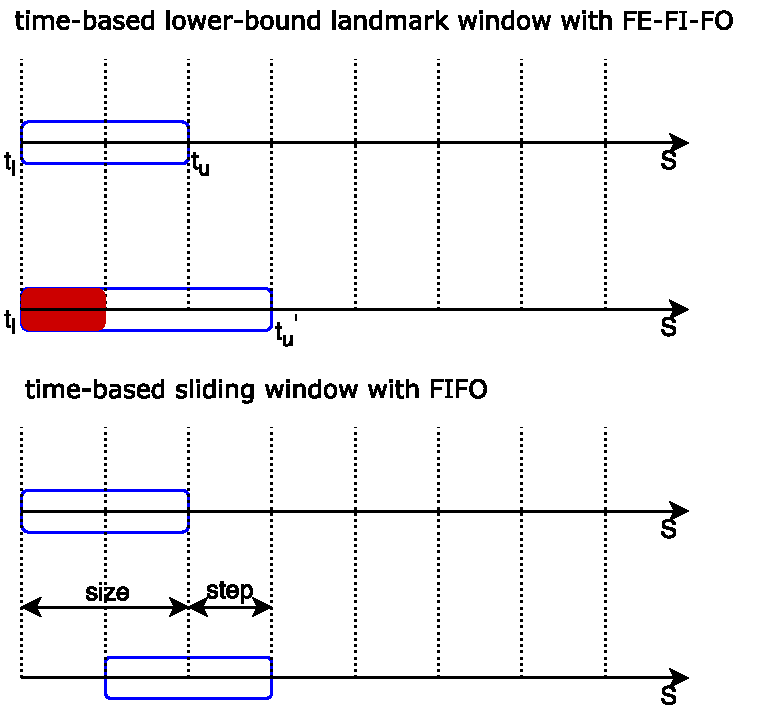
\includegraphics[width=5in]{img/3-lwcsw.pdf}
    \caption{Landmark Window Emulating Sliding Window}
    \label{fig:lwesw}
\end{figure}

Figure \ref{fig:lwesw} illustrates how the extended window semantics can emulate a logical sliding window.
A logical lower-bounded landmark window is managed with FE-FI-FO strategy.
FE-FI-FO is first expired, first in, first out, with a priority vector as $[\tau_{e}, \tau_{a}]$. 
A landmark window simulates a logical sliding window via assigning an expiration timestamp for each data item by adding the arrival timestamp with window initialization length.
This is very similar as how IMaRS \cite{barbieri2010incremental} manages the data. 
When the time reaches $t_{u'}$, the data portion marked in red will be expired in the landmark window, thus evicted. 
The content in the landmark window is the same as the sliding logical window. 

[SIZE 2s STEP 1s] is an example argument to define a logical sliding window in C-SPARQL query language \cite{barbieri2009c}.
Because this definition is only designed for the sliding window, in order to let the extended window semantics to work with the existing continuous query language, there is also a need to align the extended window semantics with the query language window definition.
This portion of work will be covered in Chapter 6. 
%
\section{Summary}
This chapter has introduced the notion of semantic importance, including the definitions, the conceptual model, the comparison rule, window management strategies and window semantics. 
The aspects in the semantic importance conceptual model are not exhaustive, and we encourage people to reuse and extend it. 
In order to make it convenient to reuse semantic importance, I have created an ontology and ground it with real world soccer examples. 
All the details are in Appendix I. 

Currently the model is consisted of two major aspects, the domain agnostic aspects and domain literate aspects. 
Domain agnostic aspects include query participation and provenance.
This is because queries are often executed independently, regardless of data, backgrounds or domains. 
Provenance information is often carried when data is generated. 
Domain literate aspects include trustworthiness and query relevance.
Often the trust models are dependent on the domain. 
For example, you might trust a Japanese friend to be your tour guide in Kobe but probably won't trust this friend to be the guide in New York.
There are lots of trust models that have been proposed and work well in different scenarios. 
Query relevance, in our model, is realized by applying query relevance ontology and query in the system. 
This ontology is different from the background ontology that is usually deployed before the system starts.
The background ontology encodes the essential knowledge of the domain, and is specifically focused on capturing domain knowledge that impacts querying and reasoning to answer questions. 
Query relevance ontology is focused on picking the query informed data for query execution. 
This requires a filtering SPARQL query to be executed before the target query is executed.
This filtering query matches all the irrelevant data that can be classified by some concepts encoded in the query relevance ontology. 
So that the data pool for query execution is smaller to make the target query run faster. 
If data comes with trust scores, it is generally recommended to perform trust filter before the target query runs. 
Again, this is to guarantee that all the data enters into the query phase is trusted.

Using priority vector to encode semantic importance guarantees an efficient and multi-fold ranking.
Together with the comparison rule, semantic importance allows the ranking to consider different aspects comprehensively.
Weighting is a simple and intuitive way to enable ordering. However, the semantic importance is embodied in the priority vector, whose ordering is realized by the position of the item. The leftier a semantic importance item is placed in the priority vector, the more significant it is compared to other items on its right. The comparison rule in Section 3.2 has provided both theory and examples on comparing semantic importance. Weighting is parallel to priority vector. There is also a way to use weighting instead of priority vector to enable ordering, where different weights can be assigned by users who assigns their preferences over semantic importance items, then reduce it into a single value, which can be used to compare and rank data importance. Since the weighting schema is a different way, this dissertation will not focus on it. 

Different window management strategies can be enabled by semantic importance. 
Work such as \cite{dell2013correctness} considers the operation semantics in stream reasoning systems. 
Window operational semantics usually refers to the way how the query is executed in the window, how the data is consumed and evicted. 
For example, C-SPARQL executes the query when the window is full, while CQELS executes when the window receives the new data.

Table \ref{tab:wsc} provides a comparison between the sliding window semantics and extended window semantics.
From what has been shown before, the extended window semantics works seamlessly with the semantic importance enabled window management strategies. 
%